\PassOptionsToPackage{table}{xcolor}
\documentclass[xcolor=dvipsnames, aspectratio=1610]{beamer}
%{{{
\usepackage{amsmath,amssymb,graphicx,float,dsfont,fancybox}
\usepackage{BeamerColor}

%\usetheme{Warsaw}
%\usetheme[secheader]{Boadilla}
\usetheme{default}
\usecolortheme[named=DarkSeaGreen4]{structure}
    \setbeamertemplate{footline}[frame number]

\beamertemplatenavigationsymbolsempty
\useinnertheme{rectangles} % Vierecke
\setbeamertemplate{itemize items}[circle]
\setbeamertemplate{sections/subsections in toc}[circle]
\usesubitemizeitemtemplate{%
    \tiny\raise1.5pt\hbox{\color{beamerstructure}${\boldsymbol \diamond}$}%
}

\usefonttheme{default}
\usepackage{relsize}
\setbeamertemplate{blocks}[default]
\usepackage{slashed}
\usepackage{ulem}

\usepackage{amsmath}
\usepackage{amsfonts}
\usepackage{amssymb}
\usepackage{amsmath,bm}
\usepackage{wasysym}
\usepackage{color}
\usepackage{movie15}
\usepackage{appendixnumberbeamer}
\usepackage{listings}
\usepackage{hyperref}
\usepackage{exscale,relsize}
\usepackage{cancel}
\usepackage{setspace}
\usepackage{tikz}
\usetikzlibrary{decorations.pathreplacing}
\usetikzlibrary{calc,shapes.callouts,shapes.arrows}
\usetikzlibrary{shapes,snakes}
\usetikzlibrary{positioning}
\usetikzlibrary{arrows}
\usetikzlibrary{backgrounds}
\usepackage{animate}
\usepackage{graphics} 


\newcommand{\tikzmark}[1]{\tikz[overlay,remember picture] \node (#1) {};}
\newcommand{\arrowthis}[2]{
        \tikz[remember picture,baseline]{\node[anchor=base,inner sep=0,outer sep=0]%
        (#1) {\underline{#1}};
        \node[overlay,single arrow,draw=none,fill=red!50,anchor=tip,rotate=60]
        at (#1.south) {#2};}%
    }%
\newcommand{\speechthis}[2]{
        \tikz[remember picture,baseline]{\node[anchor=base,inner sep=0,outer sep=0]%
        (#1) {\underline{#1}};\node[overlay,ellipse callout,fill=blue!50]
        at ($(#1.north)+(-.5cm,0.8cm)$) {#2};}%
    }%
\newcommand{\cloudethis}[2]{
        \tikz[remember picture,baseline]{\node[anchor=base,inner sep=0,outer sep=0]%
        (#1) {\underline{#1}};\node[overlay,cloud callout,callout relative pointer={(0.2cm,-0.7cm)},%
        aspect=2.5,fill=yellow!90] at ($(#1.north)+(-0.5cm,1.6cm)$) {#2};}%
    }%
\newcommand{\pointthis}[2]{
        \tikz[remember picture,baseline]{
        \node[anchor=base,inner sep=0,outer sep=0](#1) {#1};
        \node[overlay,ellipse,fill=Cerulean!50] at ($(#1.north)+(0.2cm,-0.5cm)$) {\color{black}\tiny{#2}};}%
        }%
\newcommand{\talkabove}[3]{
        \tikz[remember picture,baseline]{
        \node[anchor=base,inner sep=0,outer sep=0](#1) {{\color{#3}#1}};
        \node[overlay,ellipse,fill=#3!50] at ($(#1.north)+(0.2cm,+0.4cm)$) {\color{black}\tiny{#2}};}%
        }%
\newcommand{\talkbelow}[2]{
        \tikz[remember picture,baseline]{
        \node[anchor=base,inner sep=0,outer sep=0](#1) {#1};
        \node[overlay,ellipse,fill=Cerulean!50] at ($(#1.north)+(0.2cm,-0.5cm)$) {\color{black}\tiny #2};}%
        }%
\newcommand{\mylabel}[3]{
        \tikz[remember picture,baseline]{
        \node[ellipse] at (#1cm,#2cm) {\color{black}\tiny #3};}%
        }%
\newcommand{\bubblethis}[2]{
        \tikz[remember picture,baseline]{\node[anchor=base,inner sep=0,outer sep=0]%
        (#1) {\underline{#1}};\node[overlay,ellipse,fill=green!50] at ($(#1.north)+(-.5cm,-1.4cm)$) {#2};}%
        }%
\definecolor{alertAcolor}{rgb}{0.9 .1 0.7}
\newcommand{\alertA}[1]{\color{alertAcolor}#1\color{Black}}
%%----------------------------------------------
%%   My Colors
\definecolor{CL68}{rgb}{0,0.5,0}
\definecolor{CL95}{rgb}{0.6,1,0.6}

\definecolor{HPScol}{RGB}{255, 170, 220} 
\definecolor{DarkLightcol}{rgb}{0,0,1} 
\definecolor{Alertcol}{rgb}{1,0.1,0.3}
\definecolor{AlertcolB}{rgb}{0.4,0.2,0.9}
\definecolor{Eqcol}{rgb}{0.1,0.4,0.7}
\definecolor{Refcol}{rgb}{0.8,0.5,0.25}
\definecolor{quitegray}{rgb}{0.5,0.5,0.5}
\definecolor{springgreen}{rgb}{0.4,0.7,0.55}
\definecolor{OmegaDMcol}{RGB}{150,255,150} 
\definecolor{grcol}{rgb}{0.5,0.5,0.5}

\def \SerpC {RoyalBlue}
\def \AC {Salmon}
\def \gC {RedOrange}
\def \SMPMC {Green}
\def \EC {Fuchsia}
\def \APEXC {Purple}
\def \HPSC {HPScol}
\def \MESAC {Cyan}
\def \DLC {DarkLightcol}
\def \OrsayC {DarkLightcol}
%%----------------------------------------------
%%   My Commands
\renewcommand{\alert}[1]{{\color{Alertcol}#1}}
\newcommand{\alertC}[1]{{\color{RoyalBlue}#1}}

\definecolor{tblcol1}{rgb}{.96,.92,.95}
\definecolor{tblcol2}{rgb}{.89,.84,.88}

\newcommand{\HS}{{\color{HScol}HS }}
\newcommand{\headcol}[1]{{\color{JungleGreen}#1}}
\newcommand{\alertB}[1]{{\color{AlertcolB}#1}}
\newcommand{\eqc}[1]{{\color{Eqcol}#1}}
\newcommand{\gr}[1]{{\color{grcol}#1}}

\newcommand{\refc}[1]{{\color{Tan}#1}}
\newcommand{\myref}[1]{{\refc{\textsuperscript{\tiny{#1}} } }}
\newcommand{\myitem}{{\color{JungleGreen}\tiny{$\blacksquare$} }}
\newcommand{\putTxt}[2]{{\color{#1}\textrm{\tiny{#2}} }}
\newcommand{\putCaps}[2]{{\color{#1}\textsc{\tiny{#2}} }}
\newcommand{\bra}[1]{\left\langle{#1}\right\vert}
\newcommand{\ket}[1]{\left\vert{#1}\right\rangle}
\newcommand{\LA}{
\includegraphics[width=0.85cm]{Figures/ArrowL.jpg}\;\;}
\newcommand{\RA}{\raisebox{-0.1cm}{
\includegraphics[width=0.85cm]{Figures/ArrowS.jpg}\;\;}}
\newcommand{\RD}{
\includegraphics[width=0.85cm]{Figures/ArrowD.jpg}\;\;}
\newcommand{\RU}{
\includegraphics[width=0.85cm]{Figures/ArrowU.jpg}\;\;}
\newcommand{\RB}{
\includegraphics[width=0.45cm]{Figures/ArrowN.jpg}\;\;}

\newcommand\mysymb{\scalebox{.4}{(}\raisebox{-1.6pt}{$-$}\scalebox{.4}{)}}

\newcommand{\citeWork}[1]{ {\scriptsize{\color{Refcol} #1  \color{Black}}}}

    \newcommand\brabar{\raisebox{-4.0pt}{\scalebox{.2}{
    			\textbf{(}}}\raisebox{-4.0pt}{{\_}}\raisebox{-4.0pt}{\scalebox{.2}{\textbf{\;)
    			}}}}

\def \azeL{ \alert{{A_0^L}}    }
\def \azeR{ \alert{{A_0^R}}    }
\def \apaL{ \alert{{A_\|^L}}   }
\def \apaR{ \alert{{A_\|^R}}   }
\def \apeL{ \alert{{A_\bot^L}} }
\def \apeR{ \alert{{A_\bot^R}} }


%%----------------------------------------------
%%   Get Started
\makeatletter
\newenvironment{customlist}[2]{
  \ifnum\@itemdepth >2\relax\@toodeep\else
      \advance\@itemdepth\@ne%
      \beamer@computepref\@itemdepth%
      \usebeamerfont{itemize/enumerate \beameritemnestingprefix body}%
      \usebeamercolor[fg]{itemize/enumerate \beameritemnestingprefix body}%
      \usebeamertemplate{itemize/enumerate \beameritemnestingprefix body begin}%
      \begin{list}
        {
            \usebeamertemplate{itemize \beameritemnestingprefix item}
        }
        { \leftmargin=#1 \labelsep=#2
            \def\makelabel##1{%
              {%
                  \hss\llap{{%
                    \usebeamerfont*{itemize \beameritemnestingprefix item}%
                        \usebeamercolor[fg]{itemize \beameritemnestingprefix item}##1}}%
              }%
            }%
        }
  \fi
}
{
  \end{list}
  \usebeamertemplate{itemize/enumerate \beameritemnestingprefix body end}%
}
\makeatother


\lstdefinestyle{myScalastyle}{
  frame=tb,
  language=scala,
  aboveskip=3mm,
  belowskip=3mm,
  showstringspaces=false,
  columns=flexible,
  basicstyle={\tiny\ttfamily},
  numbers=none,
  numberstyle=\tiny\eqc,
  keywordstyle=\bf\alertB,
  commentstyle=\gr,
  stringstyle=\headcol,
  frame=single,
  breaklines=true,
  breakatwhitespace=true,
  tabsize=3,
}


%------------------------------------------------------------------------------------------------------------
%------------------------------------------------------------------------------------------------------------
%   Begin Document
%------------------------------------------------------------------------------------------------------------
%------------------------------------------------------------------------------------------------------------
\begin{document}





\begin{frame}{why} 
\linespread{1}\Large{
\begin{minipage}{0.99\textwidth}  
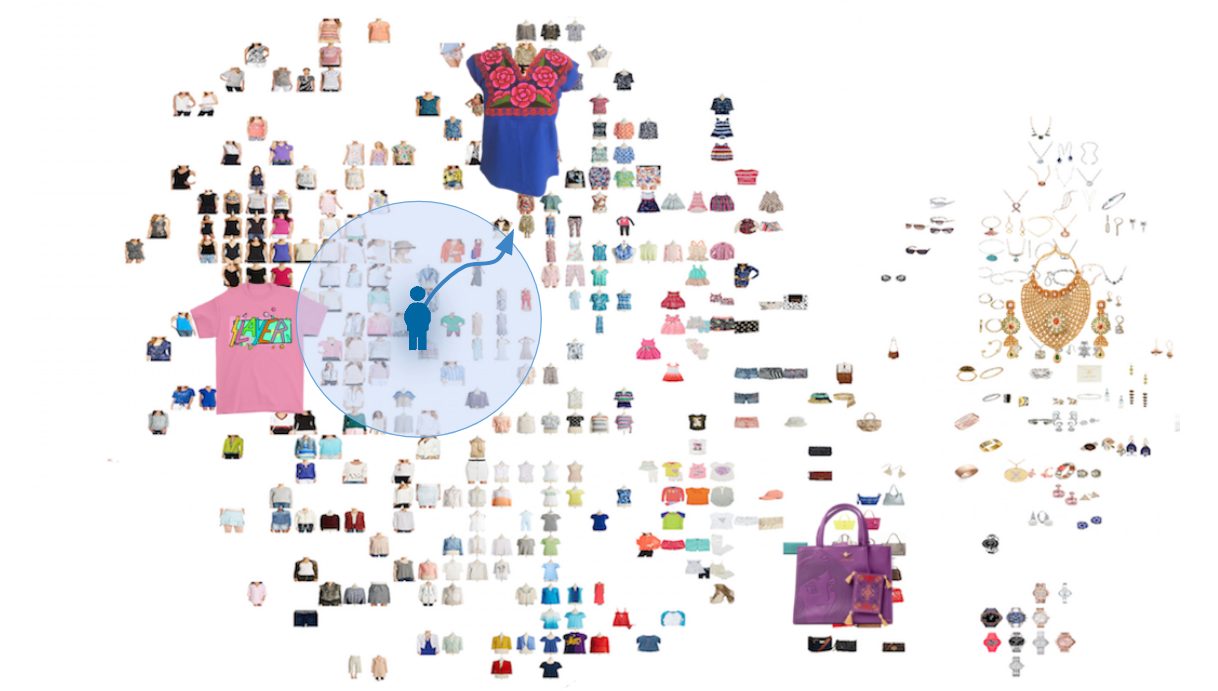
\includegraphics[width=0.8\textwidth]{Figures/vs.png}
\begin{itemize}
\item ALS find user recos after matrix factorization 
\item use currently brute force 
\end{itemize}
\RA can we improve efficiency \alertA{(talk topic)}?
\end{minipage}}
\end{frame}



\begin{frame}{nmslib contains several methods \citeWork{https://github.com/nmslib/nmslib}} 
\linespread{1}\normalsize{
\begin{minipage}{0.99\textwidth}  
\alertA{N}on \alertA{M}etric \alertA{S}pace library with focus on approximative queries.
\begin{itemize}
\item suggested by Faiss (Facebook library which is better for 1000 times bigger data)
\citeWork{https://code.facebook.com/posts/1373769912645926/faiss-a-library-for-efficient-similarity-search/}
\item many distance implementations also for text and images \RA \alertB{good as overview}
\begin{itemize}
\item  Space partitioning methods \alertB{Example 1 next slides}
\item Locality Sensitive Hashing (LSH) methods
\item Filter-and-refine methods based on projection to a lower-dimensional space
\item Filtering methods based on permutations
\item Methods that construct a proximity graph \alertB{Example 2 next slides}
\item Miscellaneous methods
\end{itemize}
\end{itemize}

\gr{All nmslib methods by name: vptree,
mvptree,
ghtree,
list\textunderscore clusters,
satree,
bbtree,
lsh\textunderscore multiprobe,
lsh\textunderscore gaussian,
lsh\textunderscore cauchy,
lsh\textunderscore threshold,
proj\textunderscore incsort,
proj\textunderscore vptree,
omedrank,
pp-index,
mi-file,
napp,
perm\textunderscore incsort\textunderscore bin,
perm\textunderscore bin\textunderscore vptree,
sw-graph,
hnsw,
nndes,
seq\textunderscore search}
\end{minipage}
}
\end{frame}



\begin{frame}{Example 1: Voronoi (e.g., Spatial Approximation tree (SA-tree)) } 
\linespread{1}\small{
\begin{minipage}{0.6\textwidth}   
\animategraphics[loop,autoplay, width=0.99\textwidth]{30}{Figures/Voronoi/Voronoi-}{0}{199}
\citeWork{https://en.wikipedia.org/wiki/Voronoi\textunderscore diagram}
\end{minipage}
\begin{minipage}{0.38\textwidth}   
rough sketch:
\begin{itemize}
\item choose generator points
\item group by closest generator point and assign index
\end{itemize}
\end{minipage}
}
\end{frame}



\begin{frame}{Example 2: SW-graph $\in$ Neighborhood Graphs} 
\linespread{1}\small{
\begin{minipage}{0.6\textwidth}  
\animategraphics[loop,autoplay, width=0.99\textwidth]{3}{Figures/nn/nn-}{0}{87}
\end{minipage}
\begin{minipage}{0.38\textwidth}  
\href{https://en.wikipedia.org/wiki/Nearest-neighbor_chain_algorithm}{\citeWork{wiki Nearest-neighbor chain algorithm}} 
 
\begin{itemize}
\item        If S is empty, choose an active cluster arbitrarily and push it onto S.
\item        Let C be the active cluster on the top of S. Compute the distances from C to all other clusters, and let D be the nearest other cluster.
\item        If D is already in S, it must be the immediate predecessor of C. Pop both clusters from S and merge them.
\item        Otherwise, if D is not already in S, push it onto S.
\end{itemize}
query similar to \href{https://de.wikipedia.org/wiki/Dijkstra-Algorithmus}{\citeWork{Dijkstra’s shortest-path}}
\end{minipage}
}
\end{frame}


\begin{frame}{what should be possible performance (glove-100-angular)} 
\linespread{1}\Large{
\begin{minipage}{0.99\textwidth}  
\citeWork{https://github.com/erikbern/ann-benchmarks (python)}

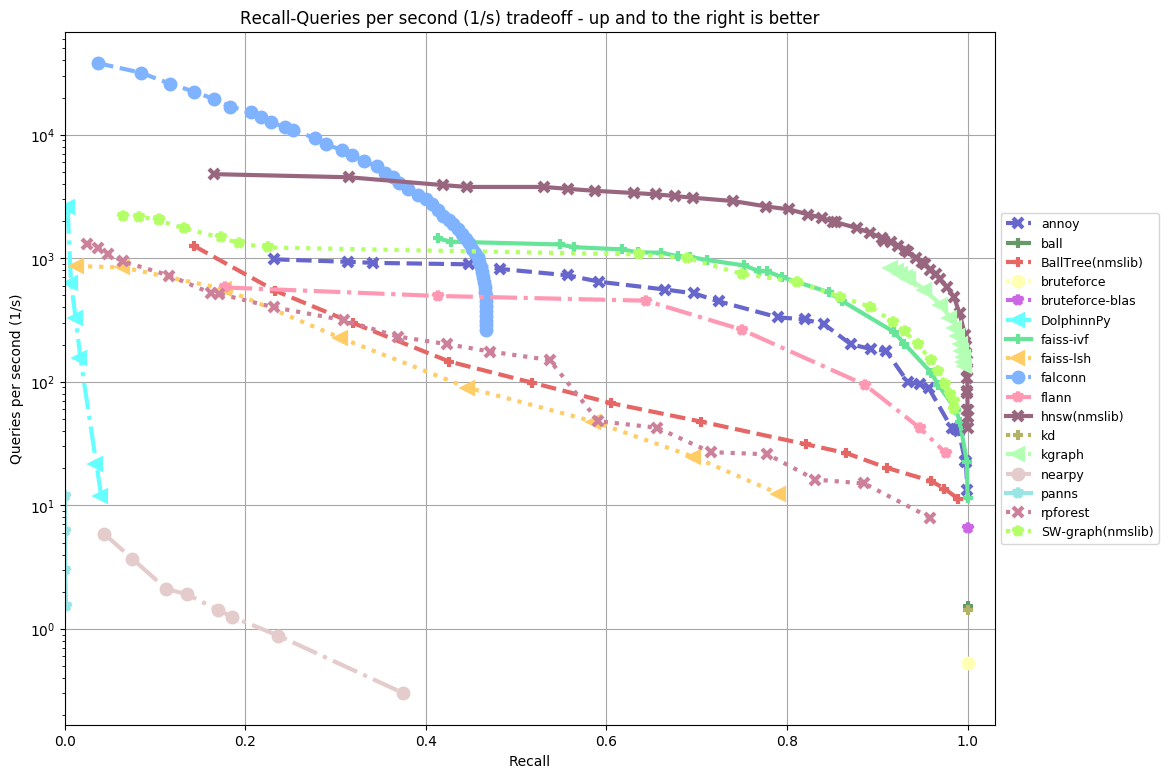
\includegraphics[width=0.8\textwidth]{Figures/perf_comp.png}

c5.4xlarge machine on AWS
\end{minipage}
}
\end{frame}


\begin{frame}[fragile]{result /nmslib/similarity\textunderscore search/release/experiment (random data, P50)} 
\linespread{1}\tiny{
\begin{minipage}{0.99\textwidth}  
{\fontsize{7}{2} \selectfont
\begin{tabular}{cccccccccccccccccc}
MethodName   & Recall & Recall@1 & RPE         & NPC & QTime & DistComp & ImprEff & ImprDist & Mem & IdxT & QPSec \\
vptree       & 1      & 1        & 1           & 0   & 21.7  & 400000   & 0.72    & 1        & 201 & 4    &  46  \\
mvp-tree     & 1      & 1        & 1           & 0   & 112.6 & 399999   & 0.14    & 1        & 137 & 2    &  9  \\
ghtree       & 1      & 1        & 1           & 0   & 25.7  & 400000   & 0.61    & 1        & 231 & 1    &  39  \\
 clusters    & 1      & 1        & 1           & 0   & 17.5  & 399898   & 0.89    & 1.00     & 122 & 489  &  57  \\
satree       & 1      & 1        & 1           & 0   & 124.7 & 400000   & 0.13    & 1        & 158 & 9    &  8  \\
omedrank     & 0.63   & 1        & 1.54        & 0   & 45.1  & 126792   & 0.35    & 3.15     & 127 & 0    &  22  \\
inverted idx & 0.41   & 1        & 2.43        & 0   & 16.6  & 20512    & 0.93    & 19.50    & 176 & 28   &  60 \\
permutation  & 1.00   & 1        & 1.00        & 0   & 19.8  & 292296   & 0.79    & 1.37     & 586 & 4    &  50 \\
perm bin     & 0.20   & 1        & 5.25        & 0   & 16.0  & 20016    & 0.97    & 19.99    & 106 & 1    &  62  \\
bin perm     & 0.21   & 1        & 5.20        & 0   & 17.1  & 20016    & 0.90    & 19.98    & 246 & 2    &  58  \\
sw-graph     & 0.06   & 0.78     & 2.37        & 14  & \alertA{\bf{0.3}}   & 1516     & 50.87   & 263.79   & 650 & 23   &  3298 \\
hnsw         & 0.19   & 0.63     & 3.01        & 10  & \alertA{\bf{0.2}}   & 897      & 77.28   & 446.16   & 652 & 105  &  4916  \\
seq search   & 1      & 1        & 1           & 0   & 14.6  & 400000   & 1.07    & 1        & 106 & 0    &  69  \\
\end{tabular}
}
\end{minipage}
\fboxsep=15pt 
\begin{minipage}{0.45\textwidth} 
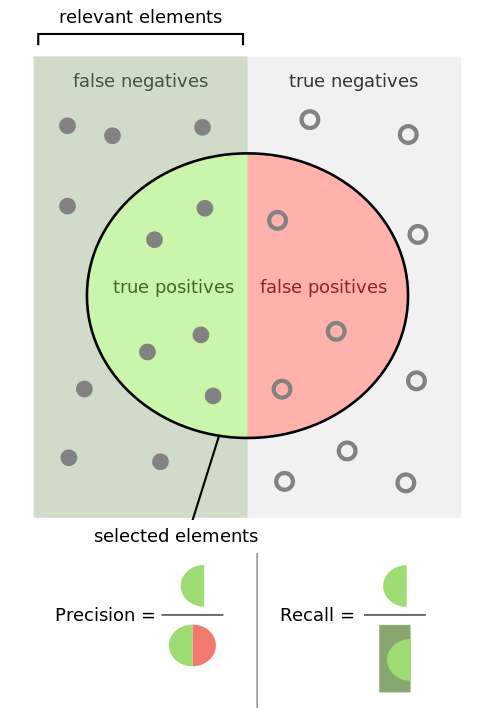
\includegraphics[width=0.6\textwidth]{Figures/Precisionrecall.png}
\end{minipage}  
\begin{minipage}{0.45\textwidth} 
\begin{itemize}
\item Recall@1: Percentage of queries for which the true nearest neighbor is returned first in the result list. ?
\item RPE: RelPosError $\frac{1}{N} \sum\limits^N_{i=1} \frac{{\rm pos} \left( o_i \right)}{i}  $ 
\item NPC: NumPointsCloser (points closer than best query return, optimal 0)
\item QTime: Query runtime [ms] 
\item DistComp: Number of distance computations.
\item ImprEff:  Improvement in runtime (improvement in efficiency) with respect to a sequential search (brute force).
\item ImprDist:  Improvement in the number of distance computations.
\item Mem:  Amount of memory used by the index and the data [MB].
\item IdxT: Index time. 
\item QPSec: Queries per second.
\end{itemize}
\end{minipage} }
\end{frame}


\begin{frame}[fragile]{result /nmslib/similarity\textunderscore search/release/experiment (tesla data, P50)} 
\linespread{1}\tiny{
\begin{minipage}{0.99\textwidth}  
{\fontsize{7}{2} \selectfont
\begin{tabular}{cccccccccccccccccc}
MethodName   & Recall & Recall@1 & RPE         & NPC & QTime & DistComp & ImprEff & ImprDist & Mem & IdxT & QPSec \\
vptree       & 1      & 1        & 1           & 0   & 15.4  & 223805   & 2.24    & 3.2      & 424 & 9     &  65  \\
mvp-tree     & 1      & 1        & 1           & 0   & 58.8  & 193013   & 0.58    & 3.7      & 317 & 4     &  17  \\
ghtree       & 1      & 1        & 1           & 0   & 53.2  & 504958   & 0.65    & 1.4     & 1569 & 29    &  19  \\
 clusters    & 1      & 1        & 1           & 0   & 16.8  & 243877   & 2.10    & 2.9      & 282 & 1662  &  59  \\
satree       & 1      & 1        & 1           & 0   & 99.6  & 277970   & 0.36    & 2.6      & 446 & 16    &  10  \\
omedrank     & 0.98   & 1        & 1.02        & 0   & 134.6 & 390457   & 0.27    & 1.8      & 295 & 0.7   &  7  \\
inverted idx & 0.90   & 1        & 1.11        & 0   & 30.4  & 36007    & 1.18    & 19.7     & 383 & 55    &  32 \\
permutation  & 1.00   & 1        & 1.00        & 0   & 37.5  & 307035   & 0.98    & 2.3      & 801 & 9     &  26 \\
perm bin     & 0.29   & 1        & 4.33        & 0   & 27.1  & 35511    & 1.33    & 20       & 257 & 1     &  37  \\
bin vptree   & 0.30   & 0.39     & 4.27        & 6   & 18.6  & 35511    & 1.91    & 20       & 496 & 2     &  54  \\
sw-graph     & 0.41   & 0.93     & 2.13        & 2   & \alertA{\bf{0.2}}   & 881      & 181     & 805      & 801 & 27    &  5145 \\
hnsw         & 0.51   & 0.77     & 1.86        & 17  & \alertA{\bf{0.1}}   & 370      & 305     & 1917     & 804 & 69    &  8389  \\
seq search   & 1      & 1        & 1           & 0   & 33.7  & 709910   & 1.07    & 1        & 257 & 0     &  30  \\
\end{tabular}
}
\end{minipage}
\fboxsep=15pt 
\begin{minipage}{0.45\textwidth} 
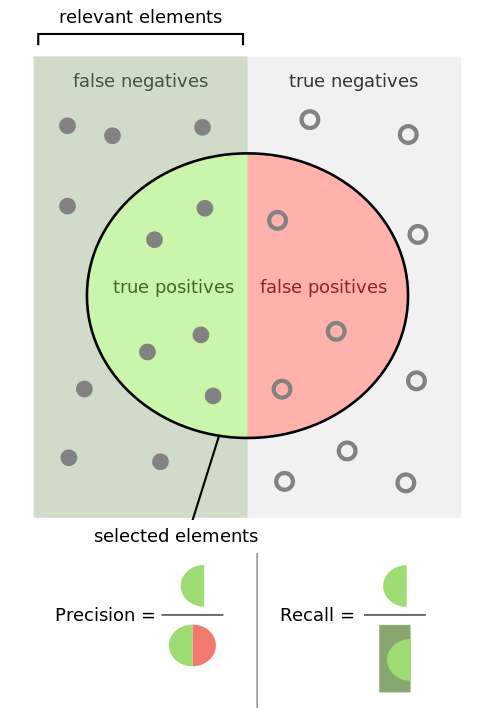
\includegraphics[width=0.6\textwidth]{Figures/Precisionrecall.png}
\end{minipage}  
\begin{minipage}{0.45\textwidth} 
\begin{itemize}
\item Recall@1: Percentage of queries for which the true nearest neighbor is returned first in the result list. ?
\item RPE: RelPosError $\frac{1}{N} \sum\limits^N_{i=1} \frac{{\rm pos} \left( o_i \right)}{i}  $ 
\item NPC: NumPointsCloser (points closer than best query return, optimal 0)
\item QTime: Query runtime [ms] 
\item DistComp: Number of distance computations.
\item ImprEff:  Improvement in runtime (improvement in efficiency) with respect to a sequential search (brute force).
\item ImprDist:  Improvement in the number of distance computations.
\item Mem:  Amount of memory used by the index and the data [MB].
\item IdxT: Index time. 
\item QPSec: Queries per second.
\end{itemize}
\end{minipage} }
\end{frame}



\begin{frame}[fragile]{result scala (https://github.com/sambackhaus/sandbox.git), P50} 
\linespread{1}\scriptsize{
\begin{minipage}{0.55\textwidth}  

\begin{lstlisting}[style=myScalastyle]
val queries: Seq[GenericQuery] = Seq(
	new KdtreeQuery("dataPath"),
	new LshQuery("dataPath"),
	new NmslibQuery("dataPath"),
	new ReferenceQuery("dataPath"))

val resultProfiles = queries.map(q => {
		System.gc()
		q.tearUp()
		val deadline: Deadline = deadlineSeconds.seconds.fromNow
		while (deadline.hasTimeLeft) {queryVectors(Random.nextInt(queryVectors.size)), 150)}
		val profile = q.getProfile()
		q.tearDown()
		profile})
\end{lstlisting}

nmslib essence:
\begin{lstlisting}[style=myScalastyle]
val pathToQueryServer = "../nmslib/query_server/cpp_client_server/query_server"
s"$pathToQueryServer -i ./$dataUrl -s l1 -m hnsw -c efConstruction=400,delaunay_type=0 -p 10000" run

val transport: TSocket = new TSocket("localhost", 10000)
transport.get.open()

val protocol: TBinaryProtocol = new TBinaryProtocol(transport.get)
val client: QueryService.Client = new QueryService.Client(protocol)

result: Seq[ReplyEntry] = client.knnQuery(nearestNeighborCount, queryString, true, false).toList
\end{lstlisting}

\end{minipage}
\hfill
\begin{minipage}{0.40\textwidth}  


\begin{flushleft}
Result (random):\\
numPoints: 400000\\
dimensions: 90\\
neighbours: 150\\

KdtreeQuery, avg query: 1606 ms\\
LshQuery, avg query: 44 ms\\
NmslibQuery, avg query: {\alertA{\bf{0.6 ms}}}\\
ReferenceQuery, avg query: 56 ms\\
\vspace{0.2cm}
Result (random):\\
numPoints: 1000000\\
dimensions: 90\\
neighbours: 150\\

KdtreeQuery, avg query: 3889 ms\\
LshQuery, avg query: 157 ms\\
NmslibQuery, avg query: {\alertA{\bf{ 0.5 ms}}} \\
ReferenceQuery, avg query: 410 ms
\vspace{0.2cm}
Result (tesla data):\\
numPoints: 709910\\
dimensions: 94\\
neighbours: 150\\

KdtreeQuery, avg query: 2244 ms\\
LshQuery, avg query: 2 ms\\
NmslibQuery, avg query: {\alertA{\bf{0.5 ms}}}\\
ReferenceQuery, avg query: 112 ms\\
\end{flushleft}
\end{minipage}
}
\end{frame}



\begin{frame}{outlook } 
\linespread{1}\small{
\begin{minipage}{0.99\textwidth}  

\begin{itemize}
\item signifficant improvement possible up to \alertA{$\mathcal O (100)$}
\item organization of data important \alertA{(random vs real)}
\item removing, adding data \& re-indexing \alertB{(seems not entirely easy)}
\item was@bi has Faiss running on the BI-Power with GPUs. Talk, e.g., to \alertB{Darius Morawiec} (vectors $\simeq 4000$ dim and several million sets)
\item 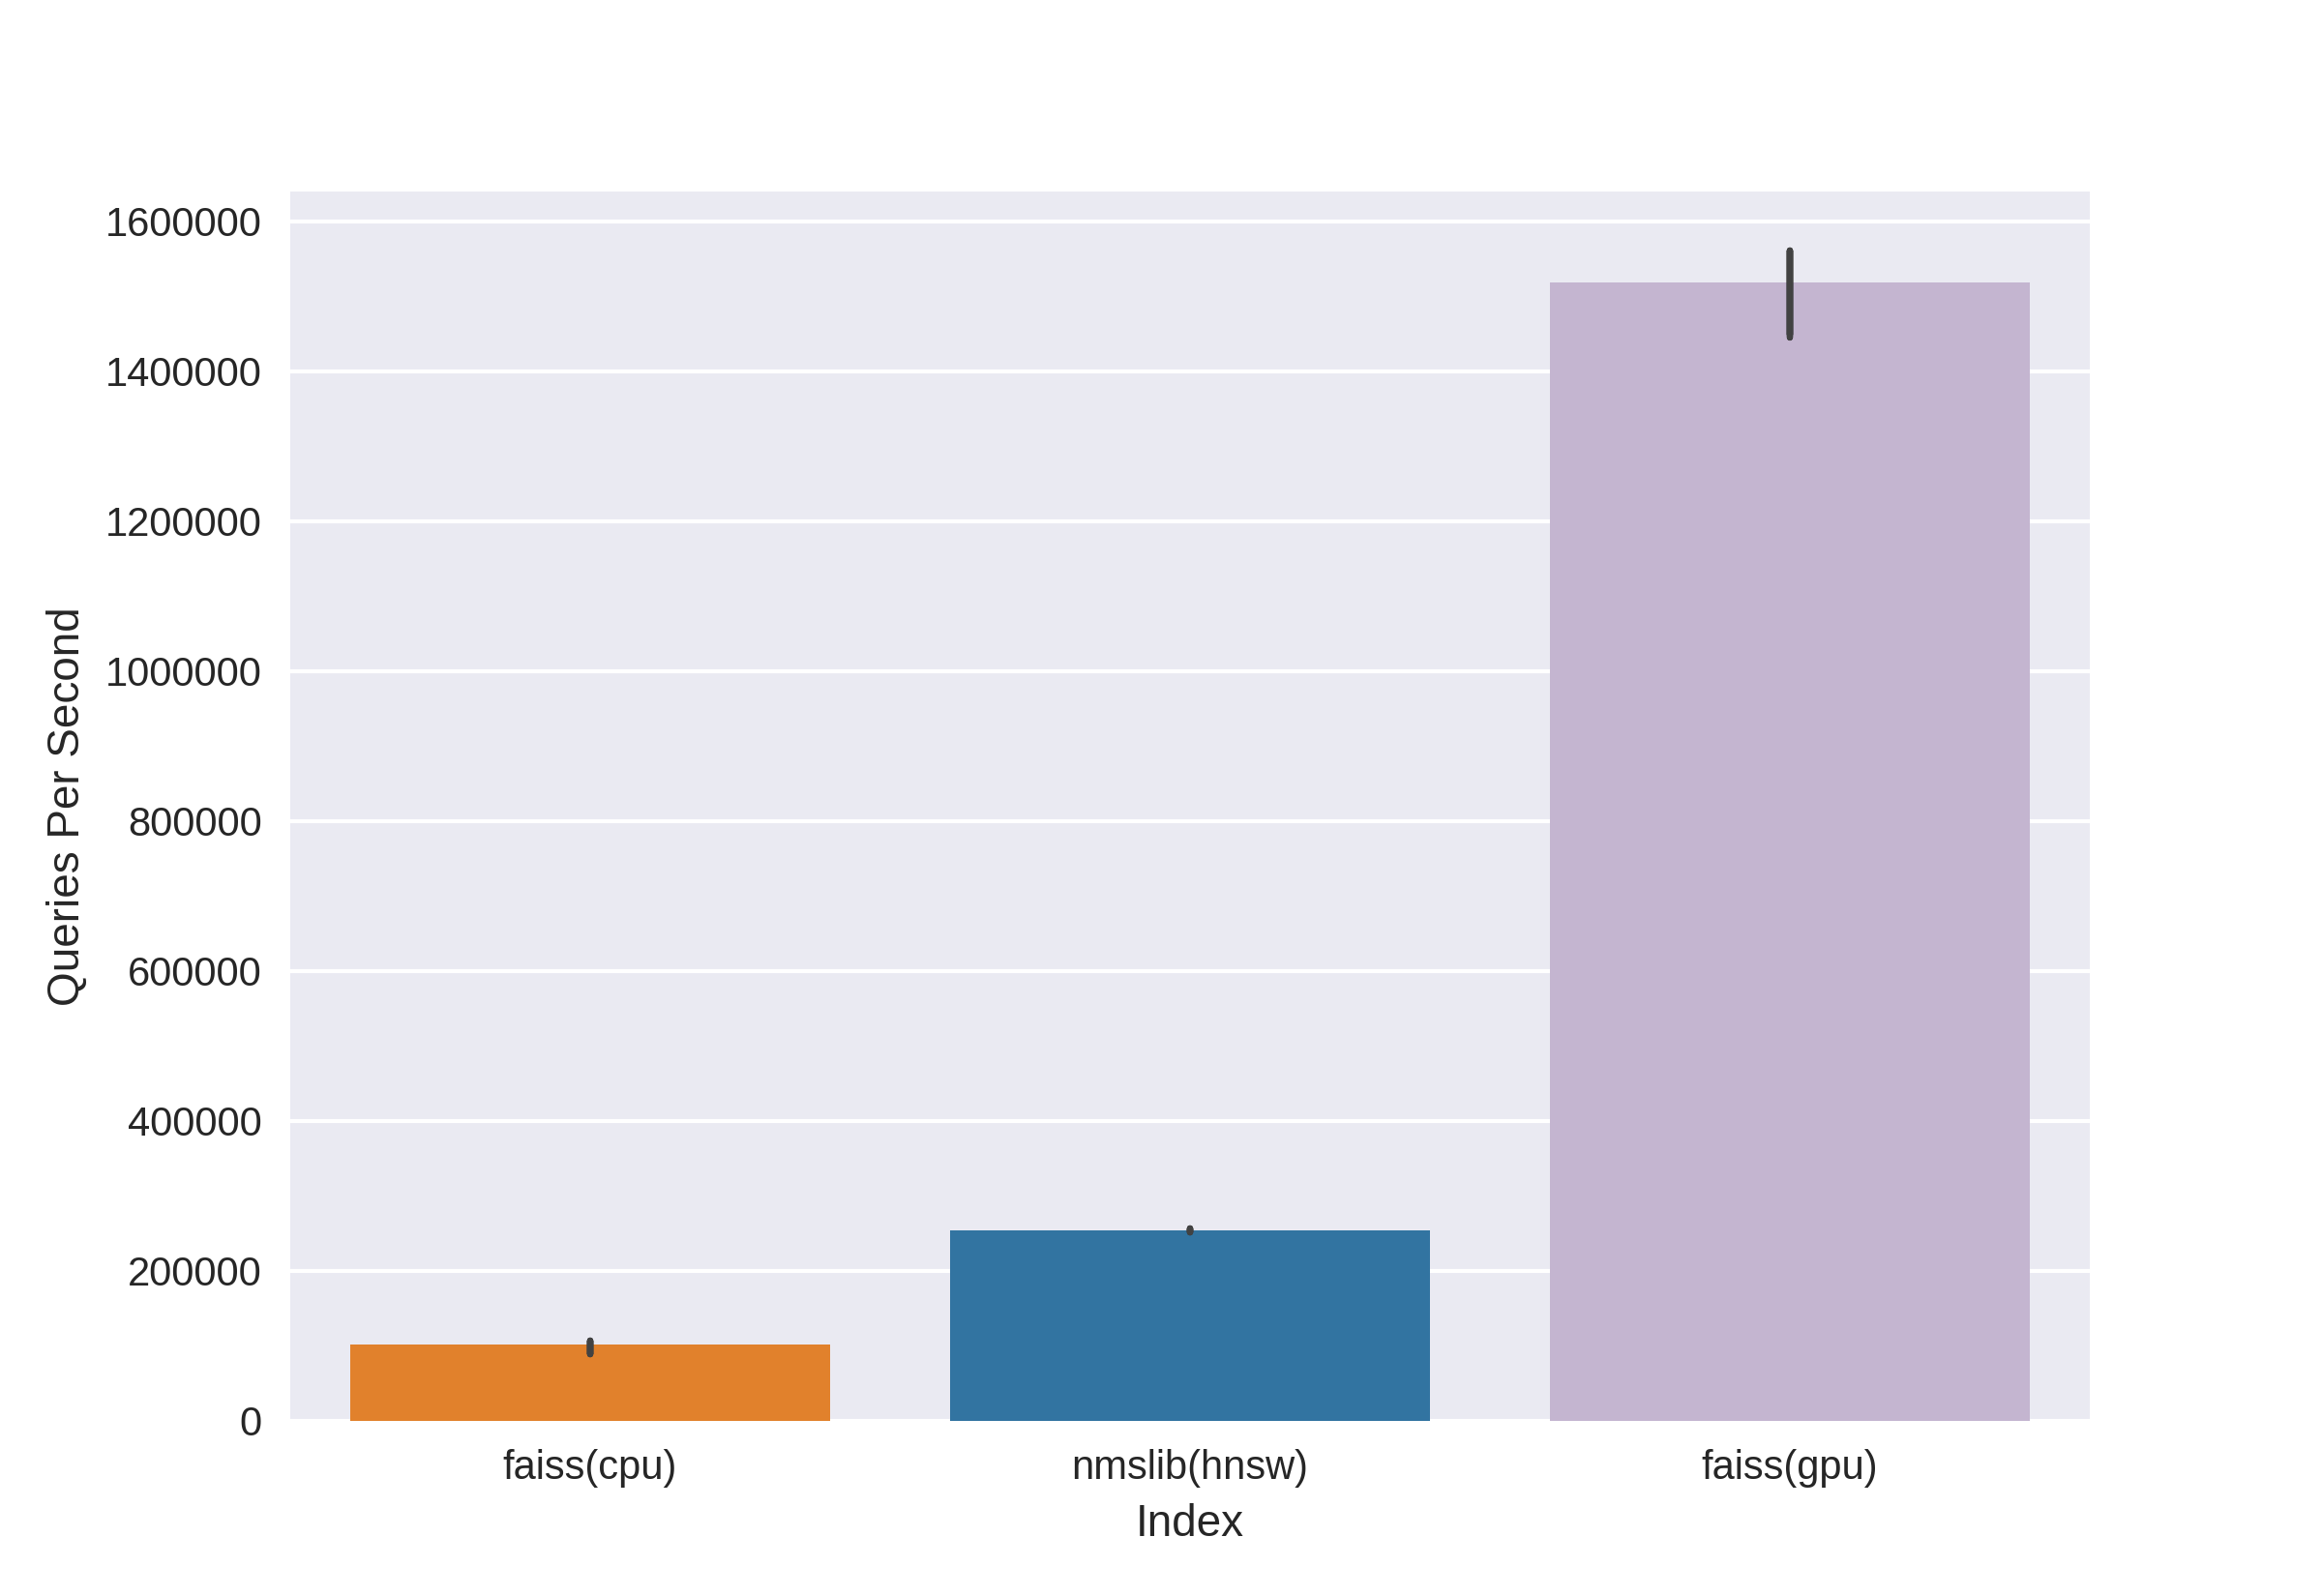
\includegraphics[width=0.4\textwidth]{Figures/faiss_gpu.png} 

\href{https://www.benfrederickson.com/approximate-nearest-neighbours-for-recommender-systems/}{\citeWork{comparison by Ben Frederickson}} \gr{(just one random benchmark)}
\end{itemize}
\end{minipage}
}
\end{frame}

\end{document}



















































